\documentclass[final,hyperref={pdfpagelabels=false}]{beamer}
\mode<presentation>{\usetheme{I6pd2}}
\usepackage[english]{babel}
\usepackage{amsmath,amsthm, amssymb, latexsym}
\usepackage[orientation=portrait,size=a1,debug]{beamerposter}
\usepackage{xcolor,colortbl}
\usepackage{tipa}
\usepackage{natbib}
\usepackage{multirow}
\usepackage{subfig}
\usepackage{tikz}
\usetikzlibrary{calc}
\usetikzlibrary{scopes}

%\usepackage{grffile}
%\usefonttheme[onlymath]{serif}
%\boldmath
% change list indention level
% \setdefaultleftmargin{3em}{}{}{}{}{}

\bibpunct[:]{(}{)}{,}{a}{}{,}
\newcommand{\ipa}[1]{\textipa{#1}} 

\usepackage{snapshot} % will write a .dep file with all dependencies, allows for easy bundling

\usepackage{array,booktabs,tabularx}
\newcolumntype{Z}{>{\centering\arraybackslash}X} % centered tabularx columns
\newcommand{\pphantom}{\textcolor{ta3aluminium}} % phantom introduces a vertical space in p formatted table columns??!!
\listfiles

%%%%
%%%%%%
\makeatletter
\define@key{beamerframe}{t}[true]{% top
  \beamer@frametopskip=.2cm plus .5\paperheight\relax%
  \beamer@framebottomskip=0pt plus 1fill\relax%
  \beamer@frametopskipautobreak=\beamer@frametopskip\relax%
  \beamer@framebottomskipautobreak=\beamer@framebottomskip\relax%
% \def\beamer@initfirstlineunskip{%
%   \def\beamer@firstlineitemizeunskip{%
%     \vskip-\partopsep\vskip-\topsep\vskip-\parskip%
%     \global\let\beamer@firstlineitemizeunskip=\relax}%
%   \everypar{\global\let\beamer@firstlineitemizeunskip=\relax}}
  \def\beamer@initfirstlineunskip{}%
}
\makeatother

\graphicspath{{figures/}}
 
\title{\huge You Should Plug Your Telemed Ultrasound to Mains Power}
\author{Pertti Palo$^{\mathrm{a}}$}
\newcommand{\emails}{$^{\mathrm{a}}$pertti.palo@taurlin.org}
\institute{Communication Sciences and Disorders, and Linguistics; University of Alberta}
\date{7th November 2026}

\newlength{\columnheight}
\setlength{\columnheight}{105cm}

\newcommand{\kommentti}[1]{{\bf[#1]}}


\begin{document}

\begin{frame}{} 
  \vspace{-1cm}
  \begin{columns}[t]
    \begin{column}{.485\linewidth}
      
      \begin{block}{Introduction}

        \begin{itemize}
          \item Ultrasound has been used for speech studies for decades
            \citep{ShawkerSonies-UltrasoundBiofeedbackSpeech-1985,Gick-UseUltrasoundLinguistic-2002,Stone-GuideAnalyzingTongue-2005}
          \item In recent years Telemed micro ultrasound devices have become
            something of a norm. 
          \item While the manual says to use mains power (connect the
            ultrasound device's power source to a wall socket) it does not say
            why, and the device will work with just power from the
            USB-connection to a computer.
          \item We discovered by accident why this recommendation exists: When running on USB
          power the ultrasound device will raise imaging power by steps during each
          recording. 
          \item According to Telemed, this is done to avoid setting off a short
          circuit panic-mode in the USB port.
          \item We report technical testing results obtained by using a bovine steak as a phantom. 
        \end{itemize}
      \end{block}
    \end{column}
      
    \begin{column}{.485\linewidth}
      \begin{block}{Methods: Recording}\footnotesize
        \begin{itemize}
          \item The conditions in the recordings were 
          \begin{itemize}
            \item {\bf without} mains power
            \begin{itemize}
              \item only air in contact with the probe -- 100 recordings 
              \item stationary phantom -- 100 recordings
              \item phantom moved manually by experimenter -- 23 recordings
            \end{itemize}
            \item {\bf with} mains power
            \begin{itemize}
              \item stationary phantom -- 13 recordings
              \item phantom moved manually by experimenter -- 25 recordings
            \end{itemize}
          \end{itemize}
          \item Data was analysed in PATKIT
            \citep{PaloEtAl-PATKITPhoneticAnalysis-2026}.
        \end{itemize}
      \end{block}
    \end{column}
  \end{columns}

  \vspace{1cm}

  \begin{columns}[t]
    \begin{column}{.99\linewidth}
      \begin{block}{Results: Image brightness} 
        \begin{figure}[!ht]
          \centering
          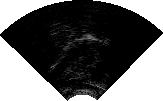
\includegraphics[width=.49\textwidth]{../figures/ultrasound_begin.png}
          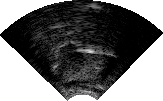
\includegraphics[width=.49\textwidth]{../figures/ultrasound_ramped_up.png}
          % generated with
        \end{figure}


        \begin{itemize}
          \item Ultrasound frames at the beginning of the recording (left) and at
            the end of the intensity ramp (right). 
          \item While neither the probe nor the phantom have moved, the image on
            the right is considerably brighter.
        \end{itemize} 
      \end{block}
    \end{column}

  \end{columns}

  \vspace{1cm}

  \begin{columns}[t]
    \begin{column}{.485\linewidth}

      \begin{block}{Results: Pixel Difference (PD) artefacts in stationary phantom} 
        \begin{figure}[!b]
          \centering
          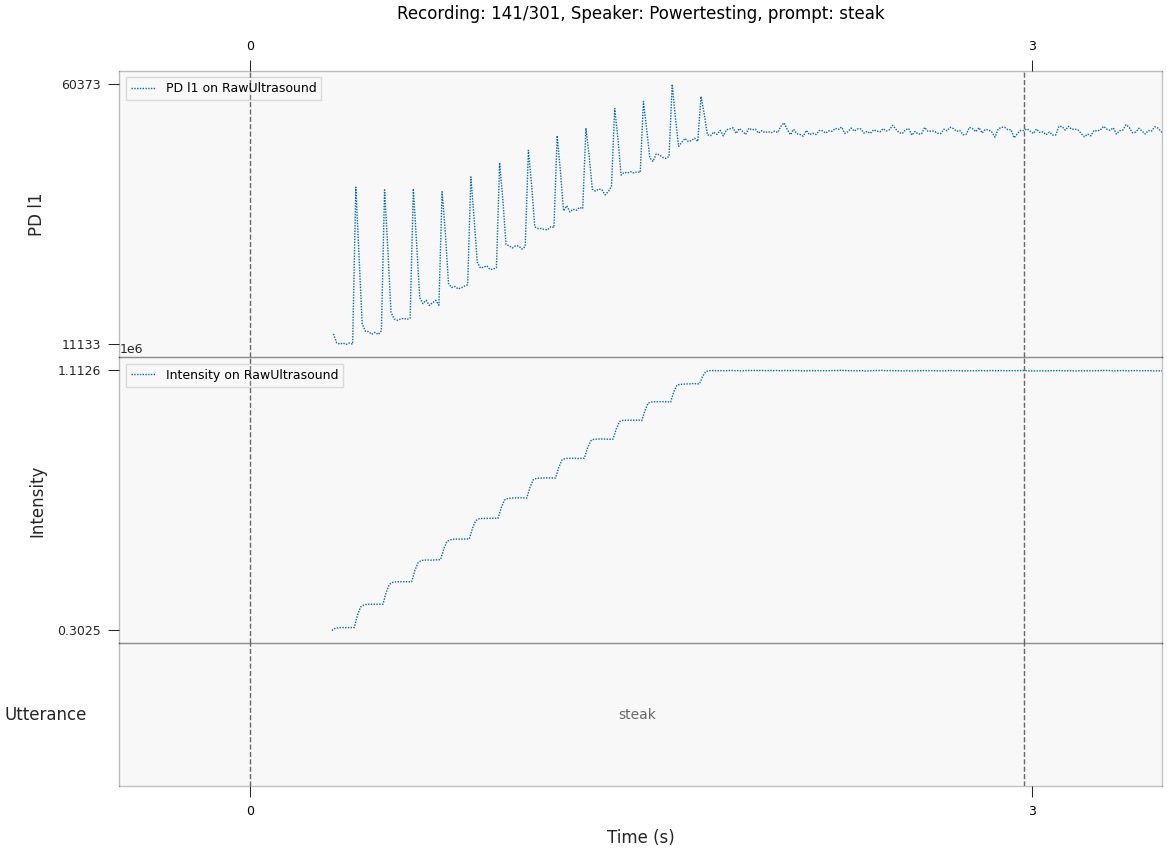
\includegraphics[width=\textwidth]{../figures/steak-no-power.png}
          % generated with
        \end{figure}

        \begin{itemize}
          \item Panels from top to bottom: Pixel Difference (PD), Image overall
            ultrasound intensity, Sound spectrogram, Sound waveform, and TextGrid
            (showing only the prompt 'hold still'). 
          \item As can be seen the image intensity ramps up by steps from
            beginning of the ultrasound recording at about $t=0.3$~s to about
            $t=1.7$~s, at which point the intensity plateaus. 
          \item There is a series of spikes in the PD curve which correspond to
            the moments when the intensity rises a step.
        \end{itemize}
      \end{block}

    \end{column}
    \begin{column}{.485\linewidth}

      \begin{block}{Results: Pixel Difference (PD) of moving phantom} 
        \begin{figure}[!b]
          \centering
          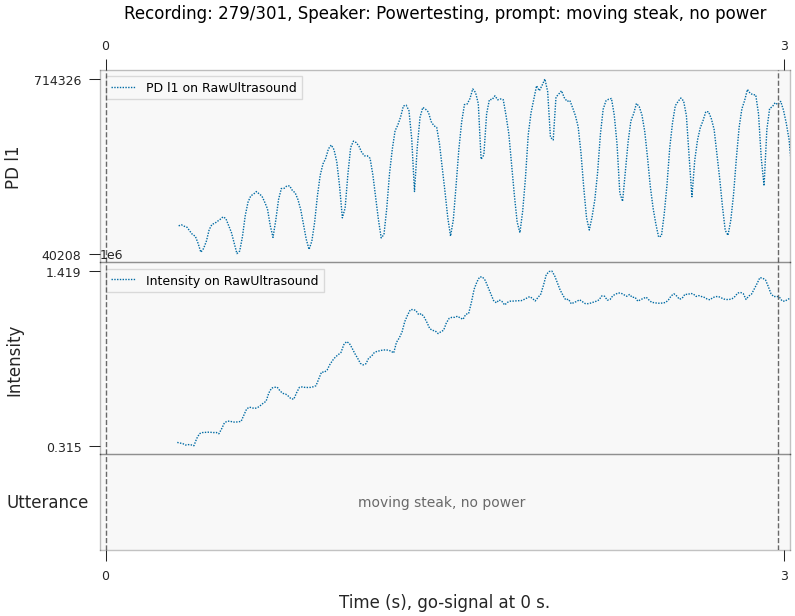
\includegraphics[width=\textwidth]{../figures/moving-steak-no-power.png}
          % generated with
        \end{figure}

        \begin{itemize}
          \item The intensity pattern remains. 
          \item Spikes in the PD curve are now hidden but the over all
          amplitude grows as intensity grows.
        \end{itemize}
      \end{block}

    \end{column}
  \end{columns}

  \vspace{1cm}

  \begin{columns}[t]
    \begin{column}{.485\linewidth}
          
      \begin{block}{Discussion: Data quality}
        \begin{itemize}
          \item Unfortunately, the stepping of intensity has consequences for
          data quality. 
          \begin{itemize}
            \item Imaging with lower power produces darker images. 
            \item In practice this means that at the beginning of the recording
            the ultrasound image will brighten in steps. 
            \item This may or may not affect anatomical tracking, and can cause
            artefacts in analysis metrics such as Pixel Difference (PD)
            \citep{Palo-MeasuringPrespeechArticulation-2019} and other analysis
            methods.
          \end{itemize}
        \end{itemize}
      \end{block}

      \begin{block}{References}

        % \footnotesize
        % This needs to be replaced by a symlink or a fresh copy.
        \bibliography{addendum,science_combined}
        \bibliographystyle{apalike}

      \end{block}
    \end{column}
    \begin{column}{.485\linewidth}

      \begin{block}{Conclusions}

        \begin{itemize}
        \item For new data: Plug the ultrasound machine into mains power
          whenever possible and if you need to run it with only USB power, make
          a note of that in your recording metadata and/or laboratory journal. 
        \item For old data, if you do not know that the device was plugged in
          to mains electricity, there are two ways of checking if there is a
          problem with data quality. 
        \item First, play a recording and look at the
          data. If the ultrasound image seems to get brighter they may be a
          problem. 
        \item Second, examine the intensity curves in PATKIT. Depending on image contents, you may need
          to look at more than one recording to see if intensity is going up
          step-wise. 
        \item In case the intensity is ramping up, any intensity based measures
          might be unreliable. 
        \item Examining only PD curves in PATKIT or AAA
          \citep{ArticulateInstruments-ArticulateAssistantAdvanced-2012-actual}
          is not reliable as seen in the moving phantom case. 
        \item Not seeing the pattern in the PD curve of a recording should not
          be taken as evidence of the absence of the problem in a dataset, nor
          even the recording in question, as it may affect event timing without
          being easily detectable. 
        \item So, plug your ultrasound to mains power.
        \end{itemize}
      \end{block}


      % \vspace*{1cm}

      % \begin{block}{Acknowledgements}
      %   %\footnotesize
      %   \begin{minipage}{0.5\textwidth}
      %     % \includegraphics[scale=1]{figures/rbo.jpg}
      %     I wish to thank Steve Cowen for assistance with the
      %     ultrasound recordings and Professor Alan Wrench for advice
      %     and help with using AAA.
      %   \end{minipage}
      %   % \begin{minipage}{0.5\textwidth}
      %   %   \hspace{10cm}\includegraphics[height=3.5cm]{figures/CASL_Sub_logo.jpg} 
      %   % \end{minipage}
      % \end{block}
    \end{column}
  \end{columns}

  
\end{frame}


\end{document}

        % {Connection with speech cycling}
        % \begin{center}
        %   \includegraphics[width=.7\columnwidth]{Fowler_cycling}
        % \end{center}
        % \begin{itemize}
        % \item Figure from \cite{Fowler:NMC:1981}.
        % \item Metronome click at 0 ms.
        % \item Relevant intervals are: 1. silence between words, 3. onset
        %   consonant, and 4. vowel.
        % \end{itemize}

        % {Future work and questions}


%%%%%%%%%%%%%%%%%%%%%%%%%%%%%%%%%%%%%%%%%%%%%%%%%%%%%%%%%%%%%%%%%%%%%%%%%%%%%%%%%%%%%%%%%%%%%%%%%%%%
%%% Local Variables: 
%%% mode: latex
%%% TeX-PDF-mode: t
%%% End:
